\section{RP13 Progressive Enhancement}
\label{sec:principle-rp13-progressive-enhancement}

Die Client-Technologien HTML und CSS haben sich über die Jahre weiterentwickelt. Dies aber immer mit dem Hintergedanken ``Progressive Enhancement''. Das bedeutet, dass die Entwicklung immer versucht hat, Rücksicht auf die älteren Browserversionen zu nehmen.
Deutlich sieht man es bei dem neuen HTML5 Standard. Neue Formularfeldtypen wie ``tel'', ``email''wurden eingeführt. Browser die HTML5 nicht unterstützen, wechslen bei einem für sie unbekannten Typ das normale Textfeld zurück. Im Falle vom Formulartyp wird es als ``text'' interpretiert.

\begin{lstlisting}[language=HTML, caption={Formularfeld mit HTML5, welches eine Telefonnummer erwartet}, label={lst:html5TelInput}]
<input type="tel" name="telefon">
\end{lstlisting}

Natürlich gibt es keine Regel ohne Ausnahmen. Manche Tags, die im HTML5 Standard eingeführt wurden, werden überhaupt nicht beachtet. Dies kann vor allem bei Versionen kleiner als neun des Internet Explorers beobachtet werden.

\subsection*{Geplante Umsetzung}
Die Beispielanwendung soll, wie bereits in \ref{sec:requirments-engineering-nonfunctionals} erwähnt, Internet Explorer 8 und höher, Chrome 25 und höher, Firefox 19 und höher und Safari 6 und höher unterstützen.

Auch Browser auf Smartphones sollten nicht vernachlässigt werden. Hierfür sollen Safari 6 und höher und Android Browser 4.0 und höher unterstützt werden.

\subsection*{Konkrete Umsetzung}
Da alle geplanten zu unterstützenden Browser nicht HTML5 interpretieren können, musste ein kleiner Trick angewendet werden, um so die Rückwärtskompatibilität zu erhöhen. Dieser Trick heisst ``modernizr'' \cite{modernizr}, eine JavaScript-Bibliothek, welche gezielt den verwendeten Browser auf seinen Funktions- und Unterstützungsumfang von HTML5 und CSS3 überprüft. Das Resultat wird dann in einem JavaScript-Objekt gespeichert und zur Verfügung gestellt.  Zusätzlich läuft modernizr in eine kleine Schleife, um die neuen Tags (head, section, article, nav, u.w.) zu aktivieren. Das bedeutet, dass diese Tags nicht mit ``div'' ersetzt werden müssen, wie es sonst der Fall wäre.

Um diese Bibliothek einzubinden, hat man nichts weiteres zu tun als das Skript im Header hinzuzufügen.

\begin{lstlisting}[language=HTML, caption=Einbinden von modernizr \cite{roomiesLayout}, firstnumber=11, label=lst:mdernizrLayoutServer]
<link href="/stylesheets/app.css" rel="stylesheet"/>
<script src="/javascripts/lib/custom.modernizr.js"></script>
\end{lstlisting}

Mit modernizr konnte erreicht werden, dass in allen geplanten Browser alle Elementen erscheinen, wenn auch nicht immer korrekt. Nicht immer korrekt, weil im Internet Explorer 8, die Darstellung des Bildes im oberen linken Rand nicht dem entspricht, was erwartet wurde.

\begin{figure}[H]
	\centering
	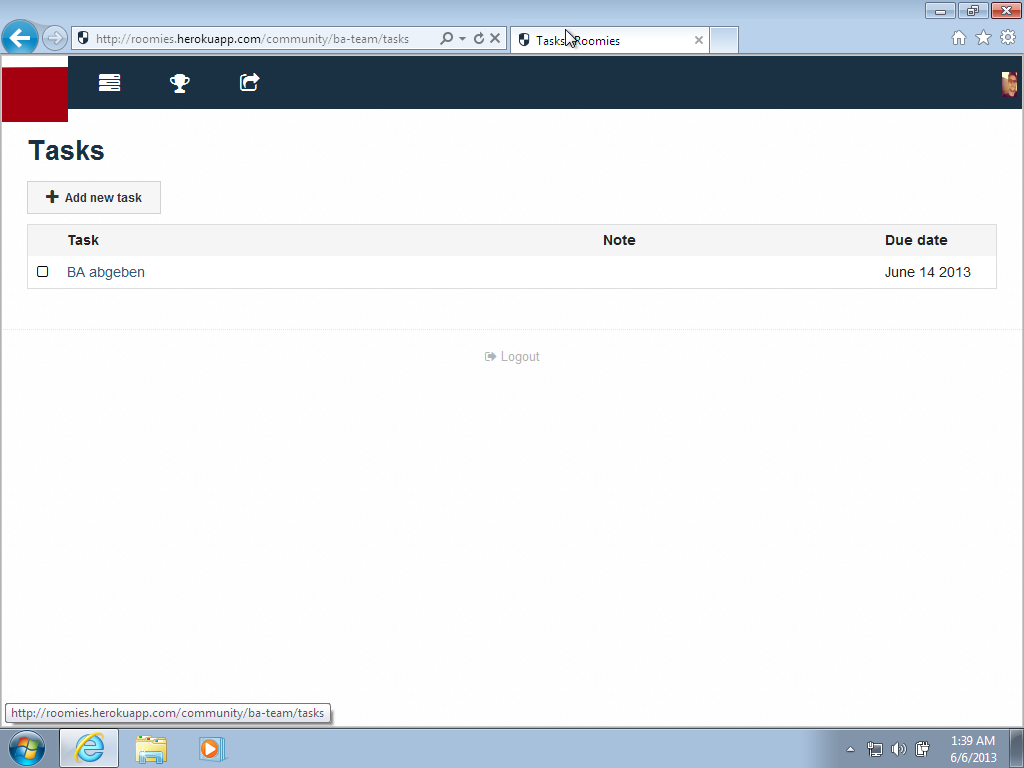
\includegraphics[width=12cm]{content/principle-demonstration/images/progressive-enhancement-ie8.png}
	\caption{Fehlerhafte Darstellung im Internet Explorer 8}
	\label{fig:iossafari-datepicker}
\end{figure}

\subsection*{Diskussion}

